\documentclass[11pt,a4paper]{report}
\usepackage[utf8]{inputenc}
\usepackage[T1]{fontenc}
\usepackage{geometry}
\usepackage{graphicx}
\usepackage{xcolor}
\usepackage{tikz}
\usepackage{pgfgantt}
\usepackage{tabularx}
\usepackage{enumitem}
\usepackage{fancyhdr}
\usepackage{hyperref}
\usepackage{amsmath}

\geometry{margin=2.5cm}

\definecolor{primaryblue}{RGB}{0,82,155}
\definecolor{secondarygreen}{RGB}{0,128,67}
\definecolor{accentgold}{RGB}{255,181,0}
\definecolor{darkgrey}{RGB}{64,64,64}

\pagestyle{fancy}
\fancyhf{}
\fancyhead[L]{\textcolor{primaryblue}{\textbf{Go-to-Market Strategy}}}
\fancyhead[R]{\textcolor{darkgrey}{AI Strategy Platform}}
\fancyfoot[C]{\thepage}

\begin{document}

\begin{titlepage}
\centering
\vspace*{2cm}


\begin{tikzpicture}
\node[draw=primaryblue, line width=3pt, minimum width=12cm, minimum height=4cm, rounded corners=10pt] (box) {};
\node at (box.center) {
    \begin{minipage}{10cm}
    \centering
    \textcolor{primaryblue}{\Huge\textbf{Go-to-Market Strategy}}\\[0.5cm]
    \textcolor{secondarygreen}{\Large UK Local Council Market Entry}\\[1cm]
    \textcolor{darkgrey}{\large Q1 2025 Launch Plan}
    \end{minipage}
};
\end{tikzpicture}

\vfill
\textcolor{darkgrey}{\large Version 1.0 | December 2024}
\end{titlepage}

\tableofcontents
\newpage

\chapter{Executive Summary}

\section{Strategic Overview}
Our go-to-market strategy focuses on establishing the AI Strategy Platform as the essential solution for UK local councils navigating AI transformation. Through a phased approach targeting early adopter councils, we will build credibility, refine our offering, and scale to nationwide coverage within 18 months.

\section{Key Success Metrics}
\begin{itemize}
\item 25 pilot councils by Q2 2025
\item 100 active councils by Q4 2025
\item £5M ARR by end of Year 1
\item 95\% customer satisfaction score
\item 3 major partnership agreements
\end{itemize}

\chapter{Market Analysis}

\section{Target Market Overview}

\subsection{Total Addressable Market}
\begin{itemize}
\item \textbf{Primary Market}: 333 principal councils in England
\item \textbf{Secondary Market}: 32 councils in Scotland, 22 in Wales, 11 in Northern Ireland
\item \textbf{Total Market Size}: 398 councils
\item \textbf{Estimated Market Value}: £150M annually
\end{itemize}

\subsection{Market Segmentation}

\begin{center}
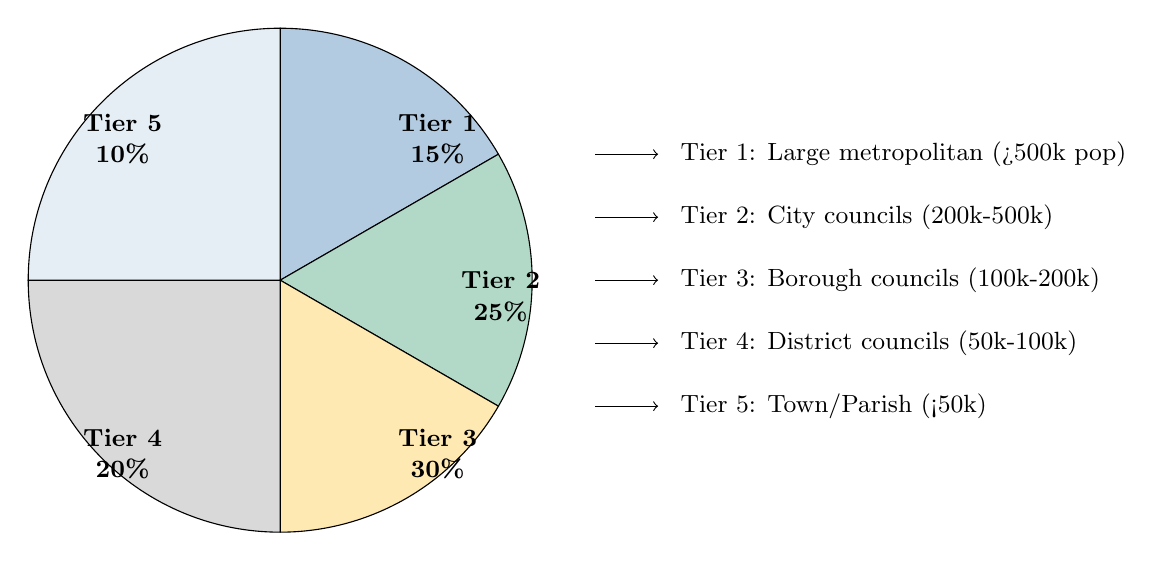
\begin{tikzpicture}[scale=0.8]
\draw[fill=primaryblue!30] (0,0) -- (0,4) arc (90:30:4) -- cycle;
\draw[fill=secondarygreen!30] (0,0) -- (30:4) arc (30:-30:4) -- cycle;
\draw[fill=accentgold!30] (0,0) -- (-30:4) arc (-30:-90:4) -- cycle;
\draw[fill=darkgrey!20] (0,0) -- (-90:4) arc (-90:-180:4) -- cycle;
\draw[fill=primaryblue!10] (0,0) -- (-180:4) arc (-180:-270:4) -- cycle;

\node at (2.5,2.5) {\small\textbf{Tier 1}};
\node at (2.5,2) {\small\textbf{15\%}};
\node at (3.5,0) {\small\textbf{Tier 2}};
\node at (3.5,-0.5) {\small\textbf{25\%}};
\node at (2.5,-2.5) {\small\textbf{Tier 3}};
\node at (2.5,-3) {\small\textbf{30\%}};
\node at (-2.5,-2.5) {\small\textbf{Tier 4}};
\node at (-2.5,-3) {\small\textbf{20\%}};
\node at (-2.5,2.5) {\small\textbf{Tier 5}};
\node at (-2.5,2) {\small\textbf{10\%}};

\draw[->] (5,2) -- (6,2);
\node[right, align=left] at (6.2,2) {\small Tier 1: Large metropolitan (>500k pop)};
\draw[->] (5,1) -- (6,1);
\node[right, align=left] at (6.2,1) {\small Tier 2: City councils (200k-500k)};
\draw[->] (5,0) -- (6,0);
\node[right, align=left] at (6.2,0) {\small Tier 3: Borough councils (100k-200k)};
\draw[->] (5,-1) -- (6,-1);
\node[right, align=left] at (6.2,-1) {\small Tier 4: District councils (50k-100k)};
\draw[->] (5,-2) -- (6,-2);
\node[right, align=left] at (6.2,-2) {\small Tier 5: Town/Parish (<50k)};
\end{tikzpicture}
\end{center}

\section{Competitive Landscape}

\subsection{Direct Competitors}
\begin{tabularx}{\textwidth}{|l|X|X|X|}
\hline
\textbf{Competitor} & \textbf{Strengths} & \textbf{Weaknesses} & \textbf{Our Advantage} \\
\hline
Big 4 Consultancies & Brand recognition, resources & High cost, generic approach & Council-specific, affordable \\
\hline
Tech Vendors & Technical expertise & Complex, not council-focused & User-friendly, sector expertise \\
\hline
Boutique Consultants & Personal service & Limited scale, inconsistent & Scalable platform, consistent quality \\
\hline
\end{tabularx}

\section{Market Readiness Indicators}
\begin{itemize}
\item 78\% of councils have digital transformation initiatives
\item £2.3B allocated for council technology upgrades 2024-2026
\item New government AI framework mandates strategic planning
\item Increasing citizen expectations for digital services
\item Growing skills gap in council IT departments
\end{itemize}

\chapter{Product Positioning}

\section{Unique Value Proposition}
"The only AI strategy platform built by local government experts, for local government needs. We transform AI complexity into clear, implementable council strategies in weeks, not months."

\section{Key Differentiators}

\begin{center}
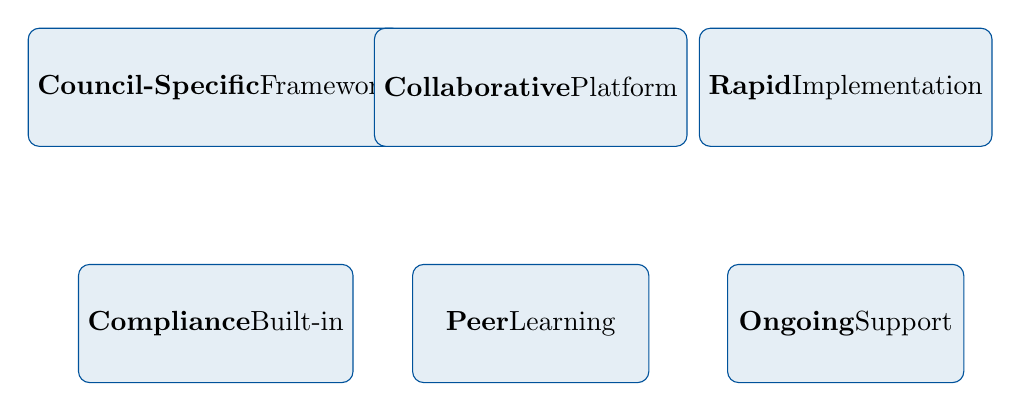
\begin{tikzpicture}[
    feature/.style={draw=primaryblue, fill=primaryblue!10, rounded corners, minimum width=3cm, minimum height=1.5cm, text centered}
]

\node[feature] (f1) at (0,0) {\textbf{Council-Specific}\\Framework};
\node[feature] (f2) at (4,0) {\textbf{Collaborative}\\Platform};
\node[feature] (f3) at (8,0) {\textbf{Rapid}\\Implementation};
\node[feature] (f4) at (0,-3) {\textbf{Compliance}\\Built-in};
\node[feature] (f5) at (4,-3) {\textbf{Peer}\\Learning};
\node[feature] (f6) at (8,-3) {\textbf{Ongoing}\\Support};

\end{tikzpicture}
\end{center}

\section{Product Tiers}

\subsection{Starter Package}
\begin{itemize}
\item AI readiness assessment
\item Basic strategy templates
\item Self-service tools
\item Community forum access
\item \textbf{Price}: £1,500/month
\end{itemize}

\subsection{Professional Package}
\begin{itemize}
\item Everything in Starter
\item Custom strategy development
\item Implementation roadmaps
\item Monthly expert consultations
\item Progress tracking dashboard
\item \textbf{Price}: £3,500/month
\end{itemize}

\subsection{Enterprise Package}
\begin{itemize}
\item Everything in Professional
\item Dedicated success manager
\item Custom integrations
\item Unlimited consultations
\item Executive workshops
\item \textbf{Price}: £7,500/month
\end{itemize}

\chapter{Launch Strategy}

\section{Phase 1: Foundation (Q1 2025)}

\subsection{Objectives}
\begin{itemize}
\item Secure 10 pilot council partnerships
\item Refine platform based on feedback
\item Build initial case studies
\item Establish market presence
\end{itemize}

\subsection{Key Activities}
\begin{itemize}
\item Beta testing with 5 friendly councils
\item Platform optimisation
\item Content creation
\item Team building
\item Partnership development
\end{itemize}

\section{Phase 2: Market Entry (Q2 2025)}

\subsection{Objectives}
\begin{itemize}
\item Official platform launch
\item 25 paying customers
\item 3 strategic partnerships
\item Strong brand awareness
\end{itemize}

\subsection{Launch Timeline}

\begin{center}
\begin{ganttchart}[
    hgrid,
    vgrid,
    x unit=0.8cm,
    y unit title=0.6cm,
    y unit chart=0.5cm,
    title label font=\small\bfseries,
    bar label font=\small,
    milestone label font=\small\color{red},
    bar/.append style={fill=primaryblue!50},
    milestone/.append style={fill=red}
]{1}{12}
\gantttitle{Q1 2025}{3} \gantttitle{Q2 2025}{3} \gantttitle{Q3 2025}{3} \gantttitle{Q4 2025}{3} \\
\gantttitlelist{1,...,12}{1} \\

\ganttbar{Beta Testing}{1}{2} \\
\ganttbar{Platform Refinement}{2}{3} \\
\ganttmilestone{Official Launch}{4} \\
\ganttbar{Marketing Campaign}{3}{6} \\
\ganttbar{Sales Outreach}{4}{9} \\
\ganttbar{Partnership Development}{2}{8} \\
\ganttbar{Customer Onboarding}{4}{12} \\
\ganttbar{Product Iteration}{5}{12} \\
\ganttmilestone{100 Councils}{10} \\
\ganttbar{Scale Operations}{7}{12}

\end{ganttchart}
\end{center}

\section{Phase 3: Growth (Q3-Q4 2025)}

\subsection{Objectives}
\begin{itemize}
\item 100 active councils
\item £5M ARR
\item National coverage
\item Category leadership
\end{itemize}

\chapter{Sales Strategy}

\section{Sales Model}

\subsection{Direct Sales Approach}
\begin{itemize}
\item Dedicated account executives for Tier 1-2 councils
\item Inside sales team for Tier 3-4 councils
\item Self-service model for Tier 5 councils
\item Average sales cycle: 3-6 months
\end{itemize}

\subsection{Sales Process}

\begin{center}
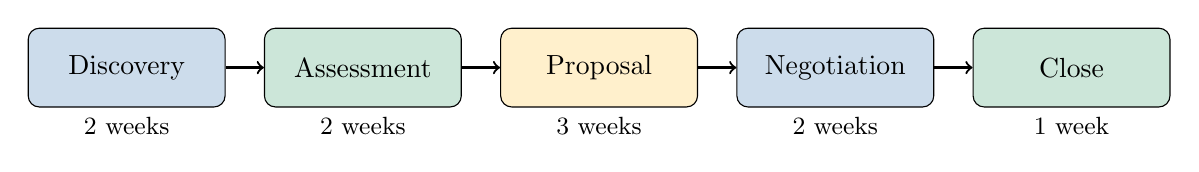
\begin{tikzpicture}[
    stage/.style={draw, rounded corners, minimum width=2.5cm, minimum height=1cm, text centered},
    arrow/.style={->, thick}
]

\node[stage, fill=primaryblue!20] (s1) at (0,0) {Discovery};
\node[stage, fill=secondarygreen!20] (s2) at (3,0) {Assessment};
\node[stage, fill=accentgold!20] (s3) at (6,0) {Proposal};
\node[stage, fill=primaryblue!20] (s4) at (9,0) {Negotiation};
\node[stage, fill=secondarygreen!20] (s5) at (12,0) {Close};

\draw[arrow] (s1) -- (s2);
\draw[arrow] (s2) -- (s3);
\draw[arrow] (s3) -- (s4);
\draw[arrow] (s4) -- (s5);

\node[below] at (s1.south) {\small 2 weeks};
\node[below] at (s2.south) {\small 2 weeks};
\node[below] at (s3.south) {\small 3 weeks};
\node[below] at (s4.south) {\small 2 weeks};
\node[below] at (s5.south) {\small 1 week};

\end{tikzpicture}
\end{center}

\section{Lead Generation}

\subsection{Inbound Channels}
\begin{itemize}
\item Content marketing (60\% of leads)
\item Webinars and events (20\%)
\item Partner referrals (15\%)
\item Website and SEO (5\%)
\end{itemize}

\subsection{Outbound Channels}
\begin{itemize}
\item Direct outreach to IT directors
\item LinkedIn campaigns
\item Conference networking
\item Council association partnerships
\end{itemize}

\chapter{Marketing Strategy}

\section{Marketing Objectives}
\begin{itemize}
\item Build brand awareness among 80\% of target councils
\item Generate 500 qualified leads in Year 1
\item Establish thought leadership position
\item Create active community of users
\end{itemize}

\section{Marketing Mix}

\subsection{Content Marketing}
\begin{itemize}
\item Weekly blog posts on AI in local government
\item Monthly whitepapers and guides
\item Quarterly research reports
\item Case studies from pilot councils
\item Video tutorials and demos
\end{itemize}

\subsection{Digital Marketing}
\begin{itemize}
\item SEO-optimised website
\item LinkedIn advertising campaign
\item Email nurture sequences
\item Retargeting campaigns
\item Social media engagement
\end{itemize}

\subsection{Events and Partnerships}
\begin{itemize}
\item Sponsor 3 major council conferences
\item Host monthly webinar series
\item Partner with council associations
\item Regional roadshow events
\item Annual user conference
\end{itemize}

\section{Marketing Budget Allocation}

\begin{center}
\begin{tikzpicture}
\pie[text=legend, radius=3]{
    30/Content Creation,
    25/Digital Advertising,
    20/Events \& Sponsorships,
    15/Partnership Development,
    10/Marketing Operations
}
\end{tikzpicture}
\end{center}

\chapter{Partnership Strategy}

\section{Strategic Partnership Types}

\subsection{Technology Partners}
\begin{itemize}
\item Microsoft: Azure integration and co-marketing
\item AWS: Cloud infrastructure and GovTech programme
\item Salesforce: CRM integration for citizen services
\end{itemize}

\subsection{Industry Partners}
\begin{itemize}
\item Local Government Association (LGA)
\item Society of Local Authority Chief Executives (SOLACE)
\item Public Sector Executive (PSE)
\item Regional improvement partnerships
\end{itemize}

\subsection{Implementation Partners}
\begin{itemize}
\item Regional consultancies
\item Systems integrators
\item Training providers
\item Change management specialists
\end{itemize}

\section{Partnership Benefits Model}

\begin{tabularx}{\textwidth}{|l|X|X|}
\hline
\textbf{Partner Type} & \textbf{We Provide} & \textbf{They Provide} \\
\hline
Technology & Integration opportunities, use cases & Technical resources, credibility \\
\hline
Industry & Thought leadership, innovation & Access, endorsement, channels \\
\hline
Implementation & Leads, platform training & Delivery capacity, local presence \\
\hline
\end{tabularx}

\chapter{Customer Success Strategy}

\section{Onboarding Programme}

\subsection{Week 1-2: Foundation}
\begin{itemize}
\item Platform setup and configuration
\item Team training sessions
\item Initial assessment completion
\item Success metrics definition
\end{itemize}

\subsection{Week 3-4: Strategy Development}
\begin{itemize}
\item Strategy workshop facilitation
\item Use case prioritisation
\item Roadmap creation
\item Stakeholder alignment
\end{itemize}

\subsection{Week 5-8: Implementation Planning}
\begin{itemize}
\item Detailed project planning
\item Resource allocation
\item Risk assessment
\item Governance framework
\end{itemize}

\section{Ongoing Support Model}

\begin{center}
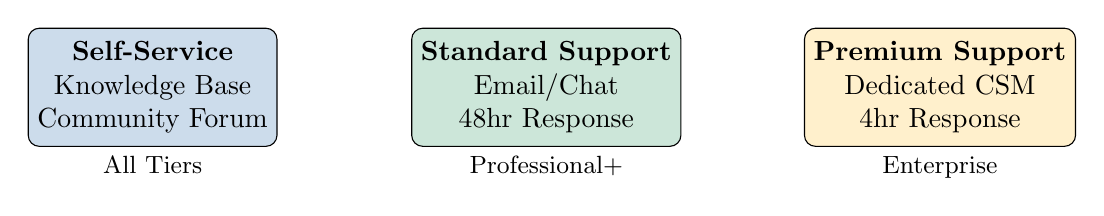
\begin{tikzpicture}[
    support/.style={draw, rounded corners, minimum width=3cm, minimum height=1.5cm, text centered, align=center}
]

\node[support, fill=primaryblue!20] (s1) at (0,0) {\textbf{Self-Service}\\Knowledge Base\\Community Forum};
\node[support, fill=secondarygreen!20] (s2) at (5,0) {\textbf{Standard Support}\\Email/Chat\\48hr Response};
\node[support, fill=accentgold!20] (s3) at (10,0) {\textbf{Premium Support}\\Dedicated CSM\\4hr Response};

\node[below] at (s1.south) {\small All Tiers};
\node[below] at (s2.south) {\small Professional+};
\node[below] at (s3.south) {\small Enterprise};

\end{tikzpicture}
\end{center}

\chapter{Financial Projections}

\section{Revenue Forecast}

\begin{center}
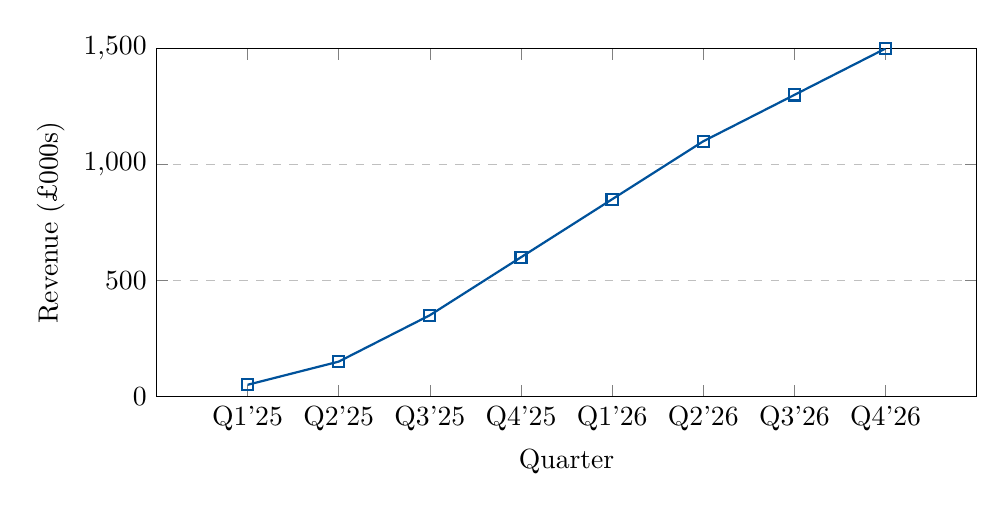
\begin{tikzpicture}
\begin{axis}[
    width=12cm,
    height=6cm,
    xlabel={Quarter},
    ylabel={Revenue (£000s)},
    xmin=0, xmax=9,
    ymin=0, ymax=1500,
    xtick={1,2,3,4,5,6,7,8},
    xticklabels={Q1'25,Q2'25,Q3'25,Q4'25,Q1'26,Q2'26,Q3'26,Q4'26},
    ymajorgrids=true,
    grid style=dashed,
]

\addplot[
    color=primaryblue,
    mark=square,
    thick
    ]
    coordinates {
    (1,50)(2,150)(3,350)(4,600)(5,850)(6,1100)(7,1300)(8,1500)
    };
    
\end{axis}
\end{tikzpicture}
\end{center}

\section{Customer Acquisition}

\begin{tabularx}{\textwidth}{|l|c|c|c|c|}
\hline
\textbf{Metric} & \textbf{Q1 2025} & \textbf{Q2 2025} & \textbf{Q3 2025} & \textbf{Q4 2025} \\
\hline
New Customers & 5 & 20 & 35 & 40 \\
Total Customers & 5 & 25 & 60 & 100 \\
MRR (£000s) & 17 & 88 & 210 & 420 \\
CAC & £8,000 & £6,500 & £5,000 & £4,500 \\
LTV:CAC Ratio & 2.5:1 & 3.2:1 & 4.1:1 & 4.5:1 \\
\hline
\end{tabularx}

\chapter{Risk Mitigation}

\section{Key Risks and Mitigation Strategies}

\subsection{Market Risks}
\begin{itemize}
\item \textbf{Risk}: Slow council adoption
\item \textbf{Mitigation}: Pilot programme with guaranteed ROI
\end{itemize}

\begin{itemize}
\item \textbf{Risk}: Budget constraints
\item \textbf{Mitigation}: Flexible pricing and phased implementation
\end{itemize}

\subsection{Competitive Risks}
\begin{itemize}
\item \textbf{Risk}: Large vendor market entry
\item \textbf{Mitigation}: Deep council relationships and specialisation
\end{itemize}

\subsection{Operational Risks}
\begin{itemize}
\item \textbf{Risk}: Scaling challenges
\item \textbf{Mitigation}: Invest in automation and partner network
\end{itemize}

\chapter{Success Metrics and KPIs}

\section{Primary KPIs}
\begin{itemize}
\item \textbf{Customer Acquisition}: 100 councils by end of Year 1
\item \textbf{Revenue}: £5M ARR by Q4 2025
\item \textbf{Customer Success}: 95\% satisfaction score
\item \textbf{Market Share}: 25\% of Tier 1-2 councils
\item \textbf{Product Adoption}: 80\% feature utilisation
\end{itemize}

\section{Leading Indicators}
\begin{itemize}
\item Website traffic and engagement
\item Content download rates
\item Webinar attendance
\item Sales pipeline velocity
\item Customer health scores
\item Platform usage metrics
\end{itemize}

\section{Reporting Dashboard}

\begin{center}
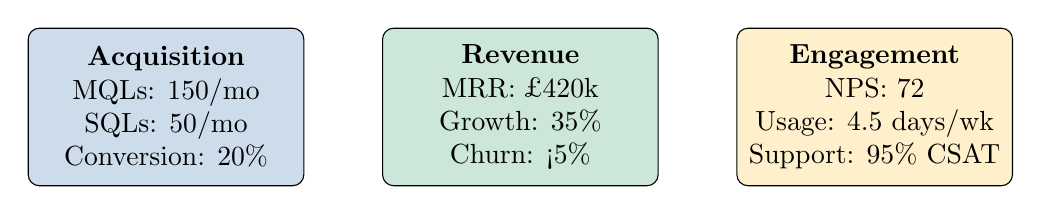
\begin{tikzpicture}[
    kpi/.style={draw, rounded corners, minimum width=3.5cm, minimum height=2cm, text centered, align=center}
]

\node[kpi, fill=primaryblue!20] (k1) at (0,0) {\textbf{Acquisition}\\MQLs: 150/mo\\SQLs: 50/mo\\Conversion: 20\%};
\node[kpi, fill=secondarygreen!20] (k2) at (4.5,0) {\textbf{Revenue}\\MRR: £420k\\Growth: 35\%\\Churn: <5\%};
\node[kpi, fill=accentgold!20] (k3) at (9,0) {\textbf{Engagement}\\NPS: 72\\Usage: 4.5 days/wk\\Support: 95\% CSAT};

\end{tikzpicture}
\end{center}

\end{document}